\let\negthickspace\undefined
\documentclass[journal,12pt,twocolumn]{IEEEtran}
\usepackage{cite}
\usepackage{amsmath,amssymb,amsfonts,amsthm}
\usepackage{algorithmic}
\usepackage{graphicx}
\usepackage{textcomp}
\usepackage{xcolor}
\usepackage{txfonts}
\usepackage{listings}
\usepackage{enumitem}
\usepackage{mathtools}
\usepackage{gensymb}
\usepackage{comment}
\usepackage[breaklinks=true]{hyperref}
\usepackage{tkz-euclide} 
\usepackage{listings}
\usepackage{gvv}                                        
\def\inputGnumericTable{}                                 
\usepackage[latin1]{inputenc}                                
\usepackage{color}                                            
\usepackage{array}                                            
\usepackage{longtable}                                       
\usepackage{calc}                                             
\usepackage{multirow}                                         
\usepackage{hhline}                                           
\usepackage{ifthen}                                           
\usepackage{lscape}
\usepackage{tfrupee}

\newtheorem{theorem}{Theorem}[section]
\newtheorem{problem}{Problem}
\newtheorem{proposition}{Proposition}[section]
\newtheorem{lemma}{Lemma}[section]
\newtheorem{corollary}[theorem]{Corollary}
\newtheorem{example}{Example}[section]
\newtheorem{definition}[problem]{Definition}
\newcommand{\BEQA}{\begin{eqnarray}}
\newcommand{\EEQA}{\end{eqnarray}}
\newcommand{\define}{\stackrel{\triangle}{=}}
\theoremstyle{remark}
\newtheorem{rem}{Remark}
\begin{document}

\bibliographystyle{IEEEtran}
\vspace{3cm}

\title{11.9.5.3}
\author{EE23BTECH11062 - V MANAS}
\maketitle
\newpage

\bigskip
\textbf{Question:}\\Let the sum of $n,2n,3n$ terms of an AP be $S_1,S_2$ and $S_3$, respectively, show that $S_3=3(S_2-S_1)$\\
\textbf{Solution:}
\begin{table}[h]
    \centering
    \begin{tabular}{|c|c|c|}
    \hline
    \textbf{Variable} & \textbf{Description}\\
    \hline
    x(0) & First term of AP\\
    \hline
    d & common difference in the AP\\
    \hline
    n & number of terms in AP\\
    \hline
    $S_k$ & sum of $k_n$ terms the AP\\
    \hline
\end{tabular}

    \caption{Variables Used}
    \label{tab:table_11.9.5.3}
\end{table}
\begin{figure}[h]
    \centering
    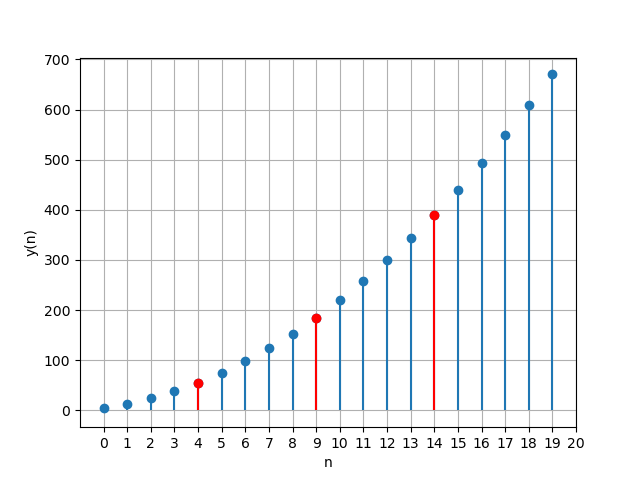
\includegraphics[width=1.1\linewidth]{figs/graph.png}
    \caption{Verification plot for the given equation}
\end{figure}\\
By equation(\ref{eq:3/ap/contour})
\begin{align}
    \implies S_1&=\frac{n+1}{2}(2x(0)+nd)u(n)\\
    \implies S_2&=\frac{2n+1}{2}(2x(0)+2nd)u(n)\\
    \implies S_3&=\frac{3n+1}{2}(2x(0)+3nd)u(n)
\end{align}
$\implies RHS=3(S_2-S_1)$
\begin{align}
    RHS&=3(\frac{2n+1}{2}(2x(0)+2nd)u(n)-\frac{n+1}{2}(2x(0)+nd)u(n))\\
    &=\frac{3n+1}{2}(2x(0)+3nd)u(n)
\end{align}
$\therefore$ LHS=RHS shows that $S_3=3(S_2-S_1)$\\
Now let we take an AP for verification,\\
Whose x0(initial term)=5,d(common difference)=3\\
$\implies$ sum of first 5 terms of the AP[y(4)]=55\\
$\implies$ sum of first 10 terms of the AP[y(9)]=185\\
$\implies$ sum of first 15 terms of the AP[y(14)]=390\\
RHS=3(y(9)-y(4))=390\\
$\implies$ y(14)=3(y(9)-y(4))\\

\end{document}
